% Figure 1: PV-Finder algorithm. Standalone TikZ; compiled by diagrams.py.
% Content follows the technical note, Section 2.2 (fig:arch) and Section 2.4.
\documentclass[tikz,border=4pt]{standalone}
\usepackage[T1]{fontenc}
\usepackage{helvet}
\renewcommand{\familydefault}{\sfdefault}
\usepackage{amsmath}
\usepackage{sansmath}
\sansmath
\usetikzlibrary{arrows.meta,positioning,calc,decorations.pathreplacing,fit,backgrounds}
\definecolor{nn}{HTML}{0072B2}
\definecolor{io}{gray}{0.55}
\begin{document}
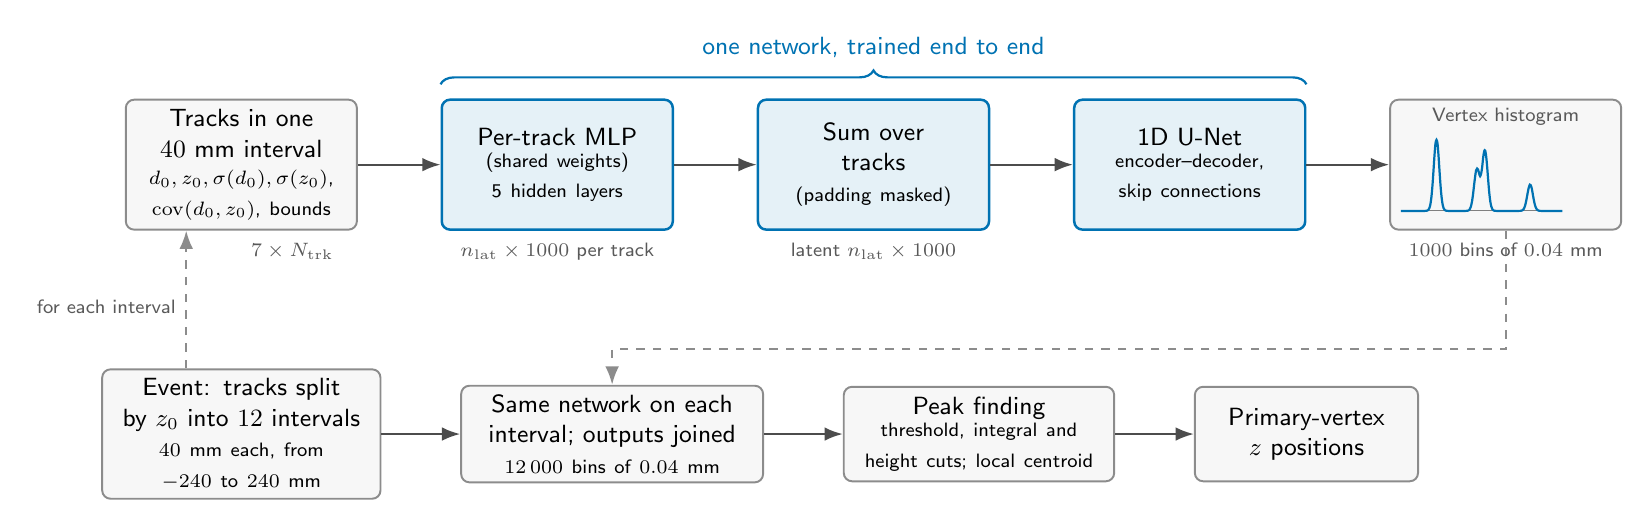
\begin{tikzpicture}[
  >=Latex, font=\small,
  box/.style={draw=io, rounded corners=3pt, fill=black!3, align=center,
              minimum height=1.65cm, text width=2.7cm, line width=0.7pt},
  net/.style={draw=nn, rounded corners=3pt, fill=nn!10, align=center,
              minimum height=1.65cm, text width=2.7cm, line width=0.9pt},
  arr/.style={->, line width=0.8pt, draw=black!70},
  dim/.style={font=\scriptsize, text=black!65},
]
  % ---- Row: one 40 mm interval -------------------------------------------
  \node[box] (trk) at (0,0)
    {Tracks in one\\$40$~mm interval\\[2pt]\scriptsize $d_0, z_0, \sigma(d_0), \sigma(z_0)$,\\\scriptsize $\mathrm{cov}(d_0,z_0)$, bounds};
  \node[net, right=1.05cm of trk] (mlp)
    {Per-track MLP\\\scriptsize (shared weights)\\\scriptsize 5 hidden layers};
  \node[net, right=1.05cm of mlp] (sum)
    {Sum over\\tracks\\\scriptsize (padding masked)};
  \node[net, right=1.05cm of sum] (unet)
    {1D U-Net\\\scriptsize encoder--decoder,\\\scriptsize skip connections};
  \node[box, right=1.05cm of unet] (hist) {};
  % Sketch of the per-interval output histogram.
  \begin{scope}[shift={($(hist.south west)+(0.15,0.25)$)}, x=2.05cm, y=0.95cm]
    \draw[black!50, line width=0.4pt] (0,0) -- (1,0);
    \draw[nn, line width=0.8pt] plot[domain=0:1, samples=160, smooth]
      (\x, {0.95*exp(-((\x-0.22)^2)/0.0006) + 0.55*exp(-((\x-0.47)^2)/0.0006)
             + 0.80*exp(-((\x-0.52)^2)/0.0006) + 0.35*exp(-((\x-0.80)^2)/0.0006)});
  \end{scope}
  \node[dim, anchor=north] at (hist.north) {Vertex histogram};

  \draw[arr] (trk) -- (mlp);
  \draw[arr] (mlp) -- (sum);
  \draw[arr] (sum) -- (unet);
  \node[dim, below=1pt of sum.south] {latent $n_{\mathrm{lat}}\times1000$};
  \draw[arr] (unet) -- (hist);

  \node[dim, below right=1pt and 0pt of trk.south] {$7\times N_{\mathrm{trk}}$};
  \node[dim, below=1pt of mlp.south] {$n_{\mathrm{lat}}\times1000$ per track};
  \node[dim, below=1pt of hist.south] {$1000$ bins of $0.04$~mm};

  % Brace over the trainable part.
  \draw[decorate, decoration={brace, amplitude=5pt}, draw=nn, line width=0.8pt]
    ($(mlp.north west)+(0,0.18)$) -- ($(unet.north east)+(0,0.18)$)
    node[midway, above=6pt, text=nn] {one network, trained end to end};

  % ---- Event level ----------------------------------------------------------
  \node[box, below=1.75cm of trk, text width=3.3cm, minimum height=1.2cm] (event)
    {Event: tracks split\\by $z_0$ into $12$ intervals\\\scriptsize $40$~mm each, from $-240$ to $240$~mm};
  \node[box, right=1.0cm of event, text width=3.6cm, minimum height=1.2cm] (stitch)
    {Same network on each\\interval; outputs joined\\\scriptsize $12\,000$ bins of $0.04$~mm};
  \node[box, right=1.0cm of stitch, text width=3.2cm, minimum height=1.2cm] (peaks)
    {Peak finding\\\scriptsize threshold, integral and\\\scriptsize height cuts; local centroid};
  \node[box, right=1.0cm of peaks, text width=2.6cm, minimum height=1.2cm] (pv)
    {Primary-vertex\\$z$ positions};

  \draw[arr] (event) -- (stitch);
  \draw[arr] (stitch) -- (peaks);
  \draw[arr] (peaks) -- (pv);
  \draw[arr, dashed, draw=black!45] ([xshift=-0.7cm]event.north) -- ([xshift=-0.7cm]trk.south)
    node[pos=0.45, left, dim] {for each interval};
  \draw[arr, dashed, draw=black!45] (hist.south) |- ($(stitch.north)+(0,0.45)$) -- (stitch.north);
\end{tikzpicture}
\end{document}
